\documentclass[a4paper]{proc}

\usepackage{amsmath}
\usepackage{amsfonts}
\usepackage{amssymb}
\usepackage{graphicx}
\usepackage{subcaption}
\usepackage{caption}

\DeclareMathOperator{\expectation}{E}

\newcommand{\euler}{\mathrm{e}}
\newcommand{\diff}{\mathrm{d}}
\newcommand{\T}{^\textup{T}}
\newcommand{\vect}[1]{\mathbf{#1}}
\newcommand{\vectGreek}[1]{\boldsymbol{#1}}
\newcommand{\matr}[1]{\mathsf{#1}}
\newcommand{\dotdotdot}{\vphantom{.}_{\cdots}}

\begin{document}
\section{Beta prior, binomial likelihood}
\subsection{Method}
Suppose a parameter $\theta$ has a prior distribution such that
\begin{equation}
\theta\sim\textup{Beta}(1,1)
\end{equation}
and that a random variable $X$ is distributed such that
\begin{equation}
X|\theta\sim\textup{Bin}(12,\theta) \ .
\end{equation}
Then after observing $X=2$, the posterior distribution is given as
\begin{equation}
(\theta|X=2)\sim\textup{Beta}(3,11) \ .
\end{equation}
ABC was used to sample the posterior distribution where the algorithm is as followed:
\begin{itemize}
  \item Sample $\theta$ from the uniform distribution
  \item Sample $X|\theta$ from the likelihood
  \item If the sampled $X|\theta$ is equal to 2, accept $\theta$, otherwise reject.
\end{itemize}

\subsection{Results}
10,000 posterior samples were drawn from the ABC algorithm. These were compared with the true posterior distribution, as shown in Figure \ref{binomial}, using the $\chi^2$ goodness of fit test.  By repeating the experiment 50 times, the mean and standard deviation $p$-value for the $\chi^2$ test was found to be $(50\pm30)\%$. This is very strong evidence that the ABC posterior samples do estimate the posterior distribution well.

The mean and standard deviation number of rejected samples per accepted sample was estimated to $(10\pm10)$.

\begin{figure}
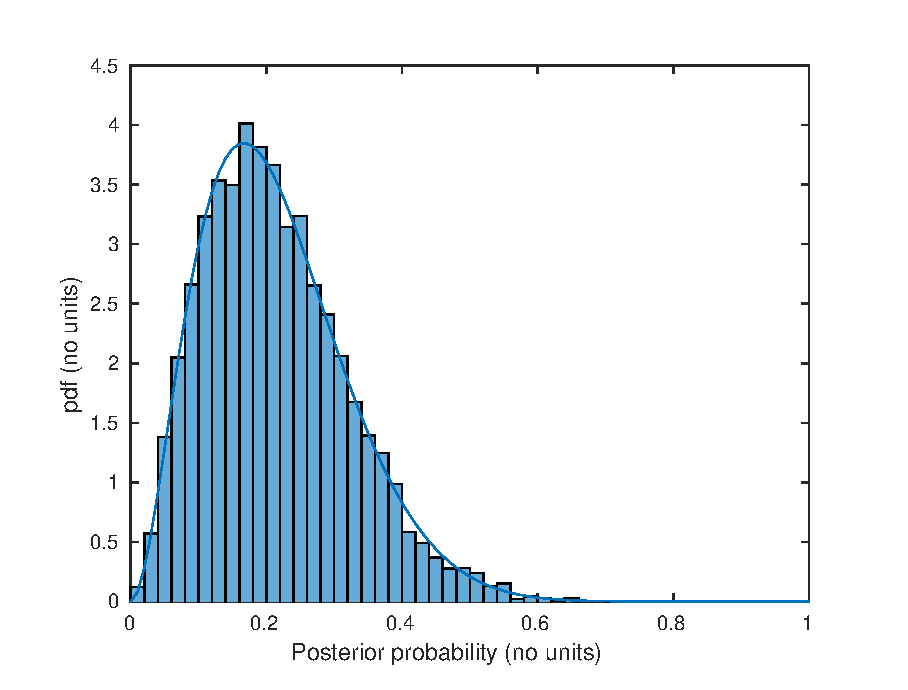
\includegraphics[width=0.5\textwidth]{binomial_ABC0528.eps}
\caption{Histogram of 10,000 posterior samples of $\textup{Beta}(3,11)$ using ABC. The curve shows the exact posterior distribution function. The $p$-value for the $\chi^2$ goodness of fit test in this example was $5\%$ to one significant figure.}
\label{binomial}
\end{figure}

\section{Normal-Gamma prior, Normal likelihood}

\subsection{Method}
Suppose the parameters $\theta$ and $\tau$ have a prior distribution such that
\begin{equation}
\tau\sim\textup{Gamma}(\alpha_0,\beta_0)
\end{equation}
and
\begin{equation}
\mu|\tau\sim\textup{N}\left(\mu_0,1/(\nu_0\tau)\right) \ .
\end{equation}
In other words, the joint prior distribution is such that
\begin{equation}
\mu,\tau\sim\textup{NGamma}(\mu_0,\nu_0,\alpha_0,\beta_0) \ .
\end{equation}
Let a random variable $X$ given the prior be distributed such that
\begin{equation}
X|\mu,\tau\sim\textup{N}(\mu,1/\tau) \ .
\end{equation}

After observing $n$ samples of $X$, labelled $x_1,x_2,\dotdotdot ,x_n$, the joint posterior distribution is given as
\begin{multline}
(\mu,\tau|X=\{x_1,\dotdotdot ,x_n\})\sim\textup{NGamma}
\left(
	\mu_1,
	\right.\\\left.
	\nu_1,
	\alpha_1,
	\beta_1
\right) \ .
\end{multline}
where the posterior parameters are
\begin{align}
\mu_1 &= \dfrac{n\bar{x}+\nu_0\mu_0}{n+\nu_0} \\
\nu_1 &= n+\nu_0 \\
\alpha_1 &= \dfrac{n}{2}+\alpha_0 \\
\beta_1 &= \beta_0+\dfrac{S_{xx}}{2}+\dfrac{n\nu_0(\bar{x}-\mu_0)^2}{2(n+\nu_0)} \ ,
\end{align}
$S_{xx}$ is the sum of squared difference from the mean and $\bar{x}$ is the sample mean.

The marginal posterior distribution is given as
\begin{equation}
(\mu|X=\{x_1,\dotdotdot ,x_n\}) = \sqrt{\dfrac{\beta_1}{\alpha_1\nu_1}} T_{2\alpha_1}
+ \mu_1
\end{equation}
and
\begin{multline}
(\tau|X=\{x_1,\dotdotdot ,x_n\}) \sim \textup{Gamma}\left(
\alpha_1,\beta_1
\right)
\end{multline}
where $T_{2\alpha}\sim t_{2\alpha}$.

ABC can be used to sample the posterior distribution but only approximately due to the arbitrary choice of comparing two samples of continuous random variables. Here, the observed and simulated samples from ABC were compared by means of hypothesis testing on the sample mean and sample standard deviation. That is, the the posterior accept/reject sampling scheme is as followed:
\begin{itemize}
	\item Sample $\tau\sim\textup{Gamma}(\alpha_0,\beta_0)$
	\item Sample $\mu|\tau\sim\textup{N}\left(\mu_0,1/(\nu_0\tau)\right)$
	\item Sample $n$ times $Y|\mu,\tau\sim\textup{N}(\mu,1/\tau)$
	\item Conduct two tailed hypothesis tests, at some confidence level $\epsilon$, on
	\begin{equation}
	\dfrac{\sqrt{n}\left(\bar{X}-\bar{Y}\right)}{\sqrt{S_X^2+S_Y^2}}\sim\textup{N}(0,1)
	\end{equation}
	\begin{equation}
	\dfrac{S_X^2}{S_Y^2}\sim F_{n-1,n-1}
	\end{equation}
	\item Accept $\mu,\tau$ if both null hypothesis are accepted, reject otherwise
\end{itemize}
where $\bar{X}$ is the sample mean and $S_X^2$ is the sample standard deviation.

\subsection{Results}
The prior parameters were set to be $\mu_0=1,\nu_0=2,\alpha_0=2,\beta_0=1$. Samples of $X$ were observed by simulating $n=10$ samples from the standard Normal distribution.

1000 posterior samples were drawn using ABC with different confidence levels for the hypothesis tests. Figure \ref{surf} shows the joint histogram of the posterior samples compared with the true posterior distribution, using a confidence level of $10\%$. By inspection, it appeared that samples from ABC is a good approximation to the posterior distribution.

The $\chi^2$ goodness of fit test was conducted on the marginal samples of the marginal posterior distribution, as shown in Figures \ref{mean} and \ref{precision}. The $p$ values for the goodness of fit test were obtained 50 times using different observations of $X$ for different confidence levels as shown in Figures \ref{pvalue_mean} and \ref{pvalue_precision}. From the figures, there is a general trend that the $p$ values increases for smaller confidence levels as expected. However the $p$ values for confidence levels $10\%$ and $20\%$ were very similar, thus there was not much improvement in the goodness of fit test when decreasing the confidence level to $10\%.$

Figure \ref{rejections} shows the number of rejections per accepted sample when using ABC. As expected, the number of rejections increases for larger confidence levels. However the magnitude of the number of rejections increased by an order of $10^2$ when decreasing the confidence level from  $20\%$ to $10\%$.

In conclusion, a confidence level of $20\%$ is good enough for ABC to approximately sample the posterior distribution. While a confidence level of $10\%$ should give a more accurate result, it suffers from very high rejection rates.

\begin{figure}
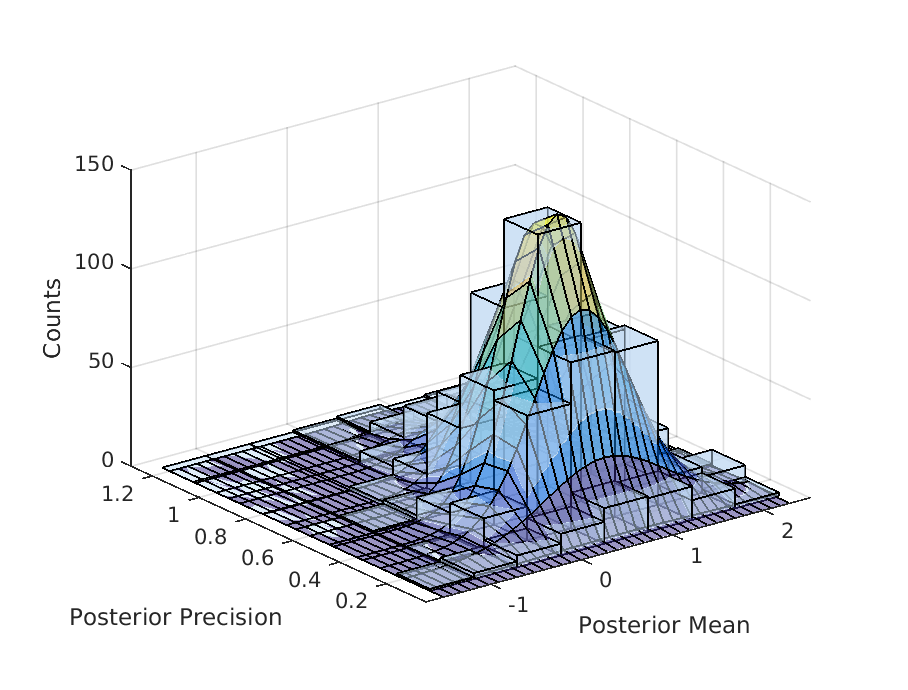
\includegraphics[width=0.5\textwidth]{surf.eps}
\caption{Joint histogram of samples of the posterior distribution using ABC compared with the true joint posterior distribution, shown as a surface plot. The confidence level was set at $10\%$ for the ABC accept/reject sampling scheme.}
\label{surf}
\end{figure}

\begin{figure}
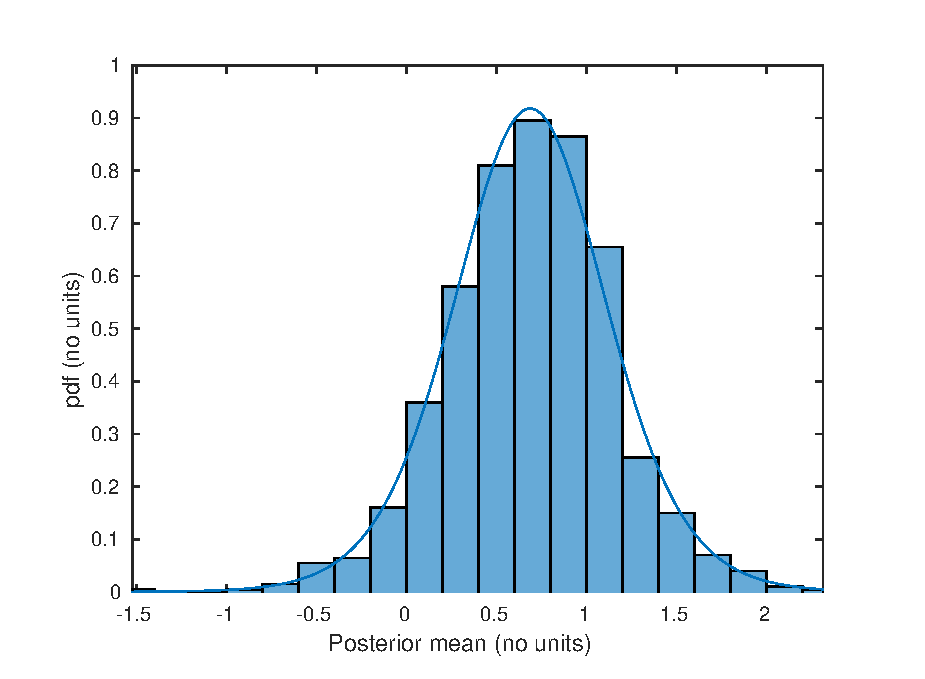
\includegraphics[width=0.5\textwidth]{mean.eps}
\caption{Marginal histogram of samples of the posterior mean, using ABC, compared with the true marginal posterior distribution. In this example, the $p$ value for the $\chi^2$ goodness of fit test was $60\%$ to one significant figure.}
\label{mean}
\end{figure}

\begin{figure}
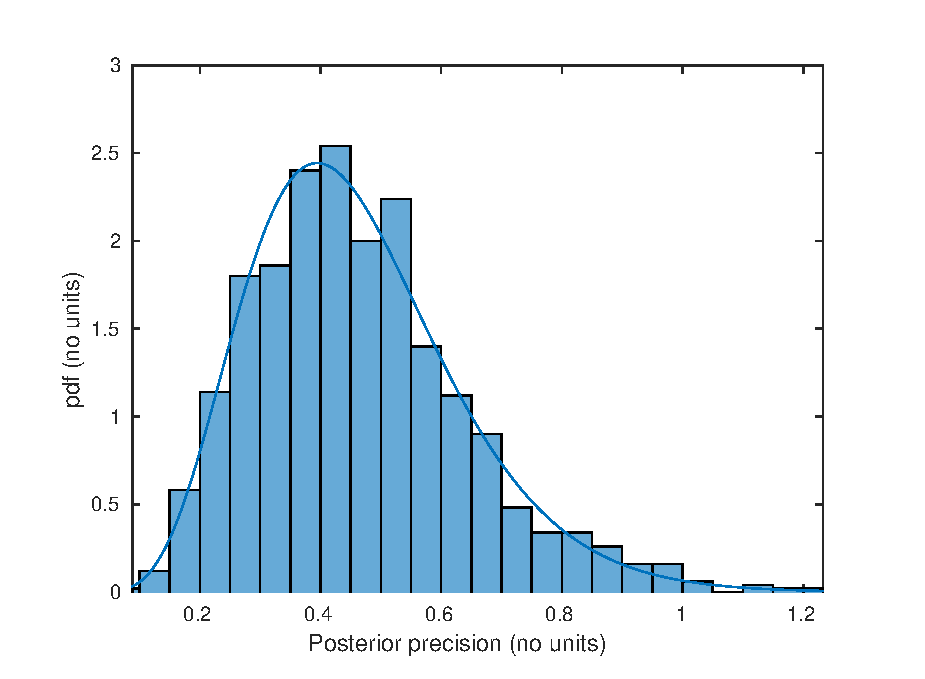
\includegraphics[width=0.5\textwidth]{precision.eps}
\caption{Marginal histogram of samples of the posterior precision, using ABC, compared with the true marginal posterior distribution. In this example, the $p$ value for the $\chi^2$ goodness of fit test was $30\%$ to one significant figure.}
\label{precision}
\end{figure}

\begin{figure}
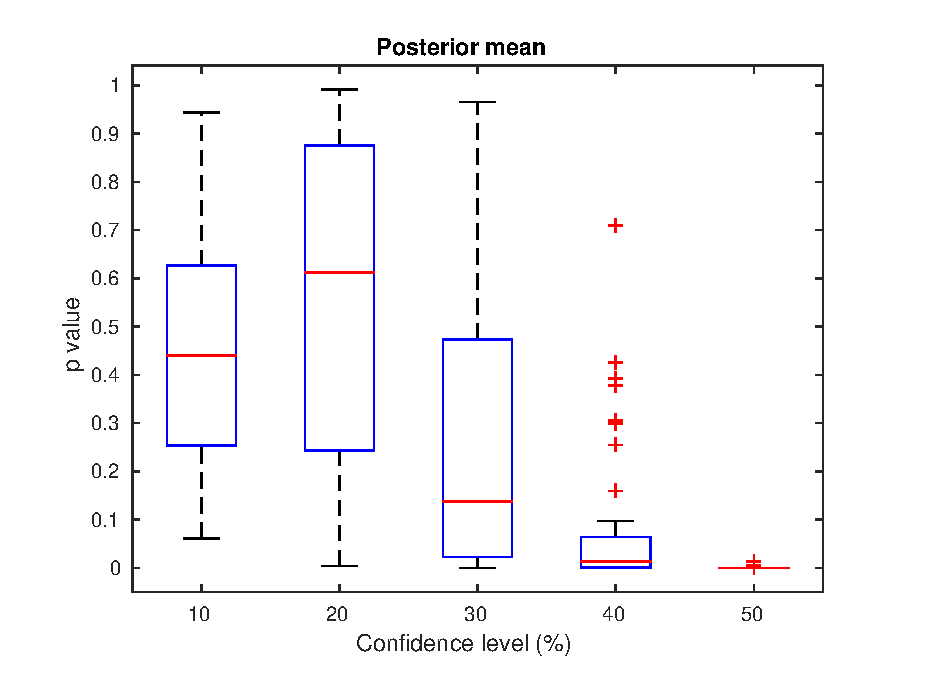
\includegraphics[width=0.5\textwidth]{pvalue_mean.eps}
\caption{$p$ values for the $\chi^2$ goodness of fit test on the marginal samples of the posterior mean. For different confidence levels, fifty $p$ values were obtained by repeating the test using different observations of the random variable $X$.}
\label{pvalue_mean}
\end{figure}

\begin{figure}
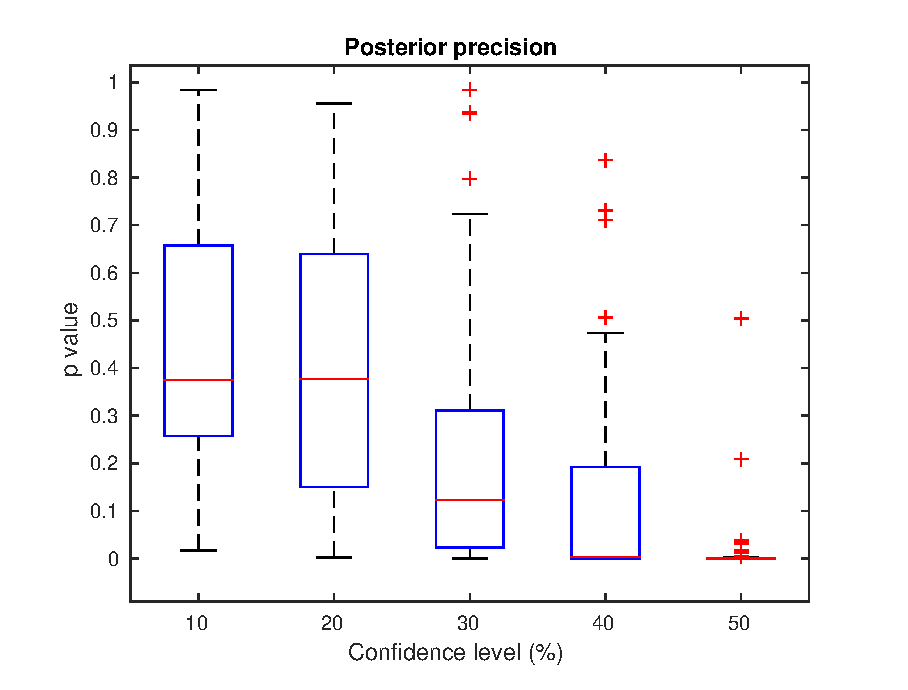
\includegraphics[width=0.5\textwidth]{pvalue_precision.eps}
\caption{$p$ values for the $\chi^2$ goodness of fit test on the marginal samples of the posterior precision. For different confidence levels, fifty $p$ values were obtained by repeating the test using different observations of the random variable $X$.}
\label{pvalue_precision}
\end{figure}

\begin{figure}
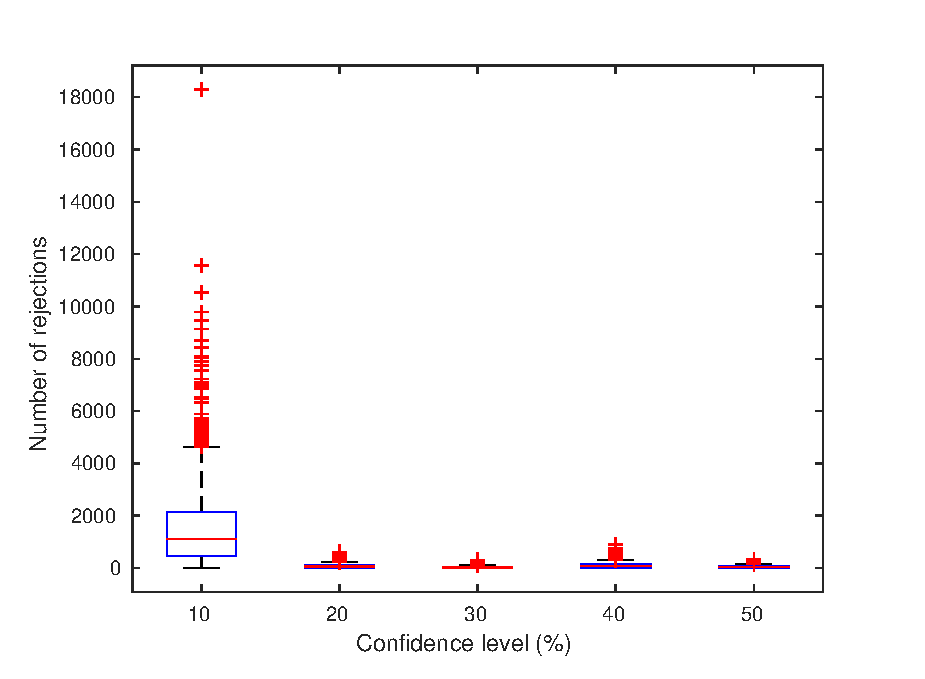
\includegraphics[width=0.5\textwidth]{rejections.eps}
\caption{The number of rejection samples per accepted sample using ABC.}
\label{rejections}
\end{figure}

\section{Evaluation}
It was found that in these ABC experiments, ABC does approximate the posterior distribution well but can suffer from high rejection rates. A good threshold is one which is small enough that samples from ABC approximate the posterior distribution well but big enough the rejection rate is feasible. It should also be noted that improper priors cannot be simulated thus cannot be used for ABC.

When the posterior distribution is not known, then there is no way to tell how well ABC approximates the posterior. The threshold can be set as small as possible, however high rejection rates will happen, especially if the prior distribution is very different to the posterior distribution.

\end{document}